\documentclass[9pt]{article}
\usepackage[utf8]{inputenc}
\usepackage{amsmath,amsthm,amsfonts,amssymb,amscd}
\usepackage{multirow,booktabs}
\usepackage{enumitem}
\usepackage{fancyhdr}
\usepackage{mathrsfs}
\usepackage{wrapfig}
\usepackage{setspace}
\usepackage{calc}
\usepackage{multicol}
\usepackage{cancel}
\usepackage{framed}
\usepackage[most]{tcolorbox}
\usepackage{tikz}
\usepackage{geometry}
\geometry{
	a4paper,
	total={170mm,257mm},
	left=20mm,
	top=20mm,
}
\title{Projectile Motion Lecture Notes}
\author{Aaron GK}
\begin{document}
	\maketitle
	\section*{Motion in 2D}
	So far, you have probably seen motion being discussed only in one dimension. However, now we will be able to see motion in two dimensions. The first one being projectile motion and the second being circular motion. Let's delve into projectiles in a little more detail.
	\subsection*{Projectile Motion} 
	Projectile motion is a motion of projectiles. Projectiles are objects that move through air without an active force. The active force could be a motive force or an engine. Projectiles go through \textbf{free fall}, meaning they have to meet the following preconditions:
	\begin{itemize}
		\item The objects must be going through \textbf{"free"} fall - meaning there is no external force supporting the motion except for gravity.
		\item \textbf{Air resistance} is to be neglected. 
	\end{itemize}
	The most interesting aspect of projectile motion is that it is two dimensional. We have motion along the X - axis as well as the Y - axis. What is even more interesting is that the motions along the X and Y axes are \textbf{independent} of one another. That makes modeling the motion very easy as we can treat the motions along the axes individually due to the independence. This rather makes studying projectiles a little boring, since it is basically doing motion in 1D, but twice(\textit{once for the X axis, another for the Y axis}). Let's look at the two 1D motions separately and what affects them. \\ \\
	Motion is affected by forces. That was the idea of Newton's Laws of Motion. Whenever there is motion, we can infer that there are forces(or lack thereof). Projectile motion is no different. To further study objects and forces acting on them, we use so-called \textbf{Free Body} diagrams that display all the forces acting on a body along with the direction of motion. Whenever we work with Free Body diagrams, we have to define axes and deal with vectors. Look at the figures below, for instance:
	\begin{center}
		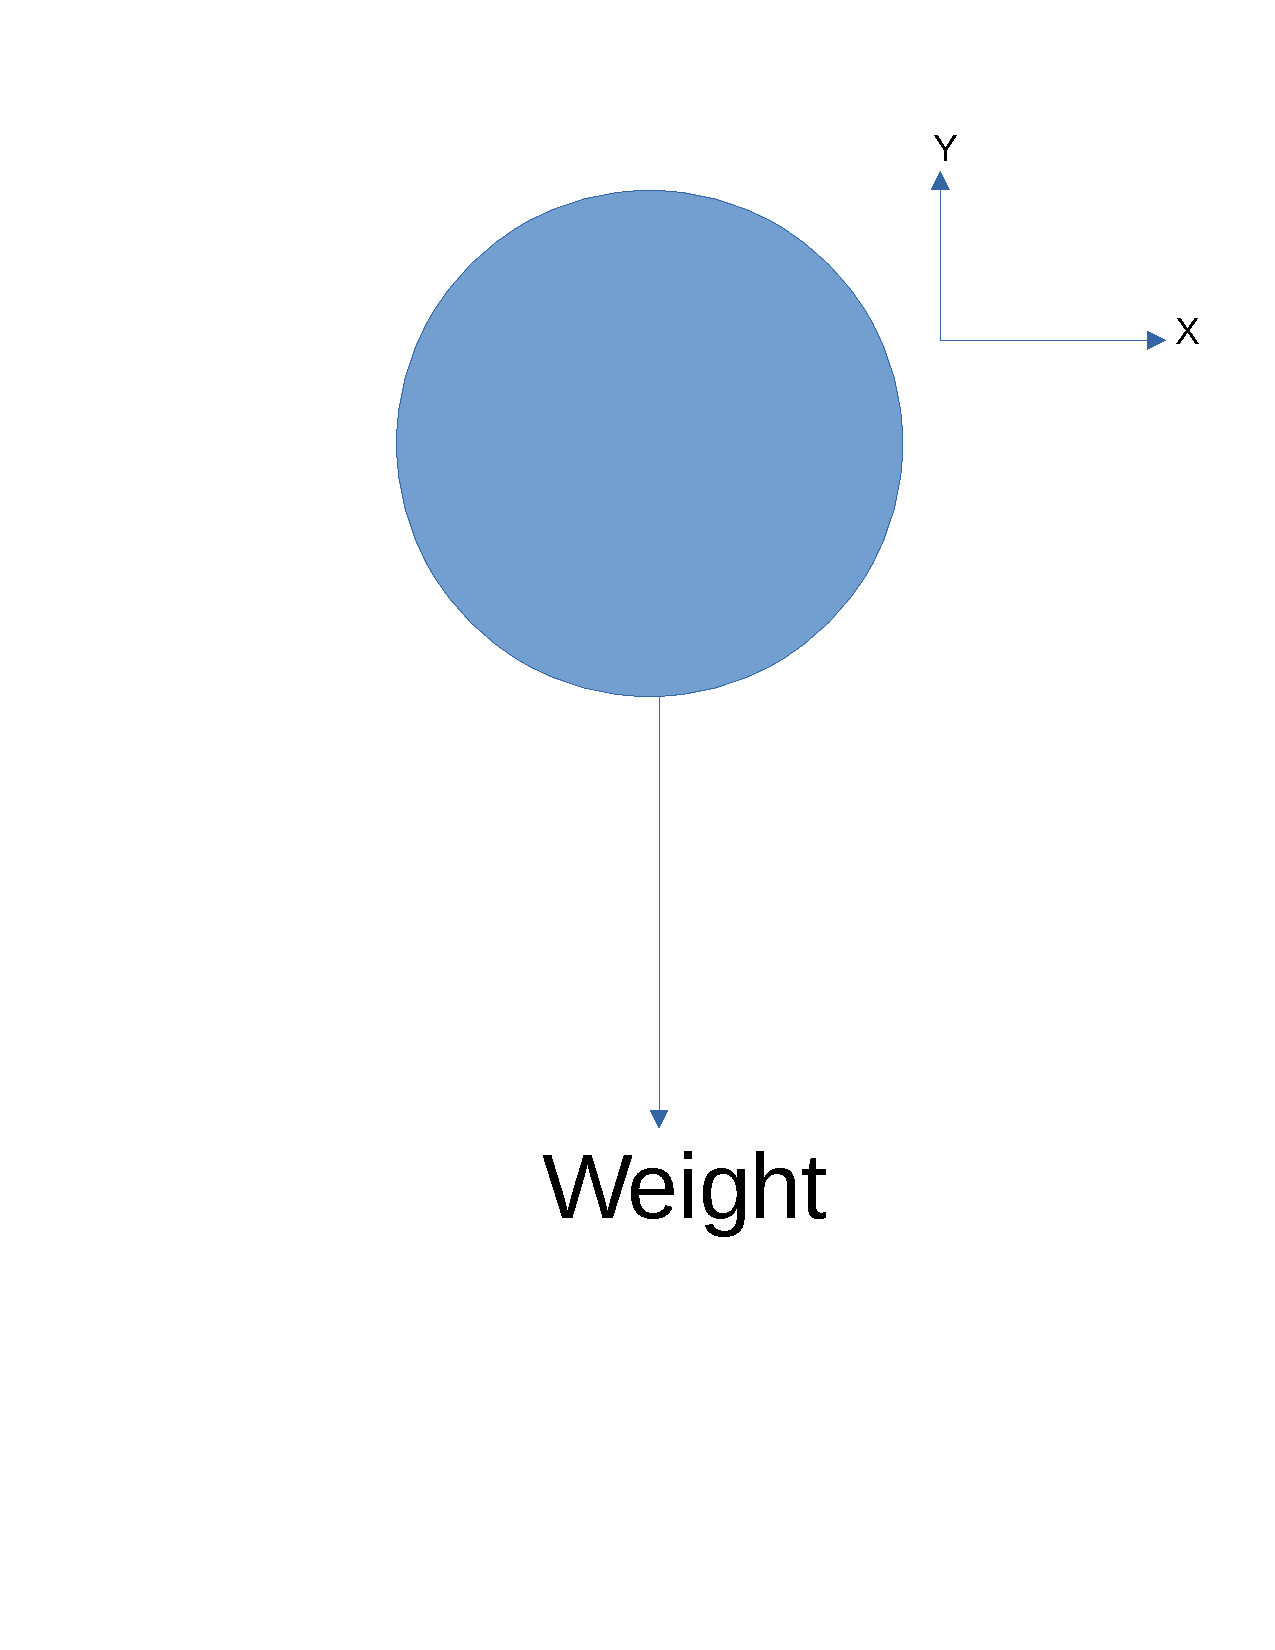
\includegraphics[scale=0.2]{projectile_free_body_diagram}
		\text{Figure - \textbf{Defining Axes}: At any point in its motion, the free body diagram for a projectile is always like the figure above.}
	\end{center}
	\subsubsection*{X - component of Projectile Motion}
	We see, from the free body diagram above, that the there is no force acting on the projectile along the X axis. We know from Newton's First Law that an object will keep its state of motion unless a net external force acts on it. Thus, our projectile's velocity along the X will be the same as the initial one through out its motion. That means, we have a Uniform motion. For uniform motion, we know the following is true:
	$$\text{V}_\text{x}=\dfrac{\text{X}}{t}$$
	\subsubsection*{Y - component of Projectile Motion}
	In our free diagram above, we see that there is only one force acting on the projectile, which is the weight of the projectile. This will make the projectile accelerate constantly resulting in a \textit{uniformly accelerated motion}. In uniformly accelerated motion the SUVAT equations apply. And they are:
	$$S=S_i+v_it+\dfrac{1}{2}at^2$$
	$$S=S_i+v_ft-\dfrac{1}{2}at^2$$
	$$S=\dfrac{v_f^2-v_i^2}{2a}$$
	$$S=v_{ave}t=(\dfrac{v_f+v_i}{2})t$$
	$$a=\dfrac{v_f-v_i}{t}$$
	\textit{We have seen in class how we can derive the equations above. Try to redo them as an exercise.}
	\subsection*{Parameters of Projectile Motion}
	Let's assume we have a projectile has a trajectory(\textit{trajectory is a fancy way of saying path}) such as the one given below.
	\begin{center}
		\includegraphics*[scale=0.15]{Projectile_Trajectory}\\
		\textit{CC-4: Wikipedia}
	\end{center}
	Since velocity is a vector, I can resolve it into its own components(vertical and horizontal). To do that, we just apply simple trigonometric knowledge.
	$$\vec{v}=\vec{v_x}+\vec{v_y}$$
	Since $\vec{v_x}$ and $\vec{v_y}$ are perpendicular, their resultant is given by Pythagoras' theorem:
	$$|\vec{v}|=\sqrt{|\vec{v_x}|^2+\vec|{v_y}|^2}$$
	To resolve, we can just use simple trig functions:
	$$\cos\theta=\dfrac{ADJ}{HYP}=\dfrac{v_x}{v}$$
	$$v_x=V\cos\theta$$
	$$\sin\theta=\dfrac{OPP}{HYP}=\dfrac{v_y}{v}$$
	$$v_y=v\sin\theta$$
	\subsubsection*{Maximum Height}
	Is the maximum vertical position attained by a projectile. Since it is a \textit{vertical} component of the motion, we can use the SUVAT equations and modify them a little to our liking.\\ \\
	Let's start with the following concepts:
	\begin{itemize}
		\item The X and Y motions of a projectile are independent, hence, we shall treat them individually.
		\item We have to define axes(or a coordinate system) since we are dealing with vectors.
		\item We have to define an origin point for our coordinate system since we need a reference frame. Usually, it is easy and conventional to use the starting point of the motion as the origin.
	\end{itemize}
	With these concepts in mind, let's start finding the $Y_{max}$. One of our SUVAT equations above was:
	$$S=\dfrac{v_f^2-v_i^2}{2a}$$
	Let's modify this and make it specific about our Y axis. We then have:
	$$y=\dfrac{v_{fy}^2-v_{iy}^2}{2a}$$
	With out definitions of the axes and the origin, we have the following be true:
	\begin{itemize}
		\item $y_i=0\text{ since we define our initial motion starting point to be the origin}$
		\item $y=y_{max}\text{ since our final destination point is the maximum height.}$
		\item The \textbf{vertical} velocity at the maximum height is 0 (\textit{why? - think of it logically(had it been non-zero, would it be our maximum height?) or using trigonometry(the angle keeps changing, and what is the angle at the maximum height?)})
		\item Depending on our axes definitions, a might be positive or negative and so does the initial velocity. If we define our axes as we did in the first figure, we have $a_y=-g$ and $v_{iy}=+v_i\sin\theta$
	\end{itemize}
	We then have:
	$$y_{max}=\dfrac{0-(v_i\sin\theta)^2}{2(-g)}$$
	$$y_{max}=\dfrac{-(v_i\sin\theta)^2}{-2g}$$
	$$y_{max}=\dfrac{(v_i\sin\theta)^2}{2g}$$
	\subsubsection*{Flight Time}
	Is the amount of time a projectile is in motion. We can usually divide this into two with the first being ascent time(\textit{time it takes to ascend to maximum height}) and second one being descent time(\textit{time it takes to descend from maximum height}). \\ \\
	Generally, we can calculate the flight time using y(t). We have seen from SUVAT equations that:
	$$S=S_i+v_it+\dfrac{1}{2}at^2$$
	We can solve the equation below to find the flight time. 
	$$y=y_i+v_{iy}t+\dfrac{1}{2}a_y-t^2$$
	However, we can simplify things by assuming that our trajectory is symmetric( \textit{that happens when the vertical coordinates of the initial and final points on the trajectory are the same}). IF I know the trajectory is symmetric, I can just find the time of ascent and multiply it by two to get the flight time. We can do that by starting from one of the SUVAT equations:
	$$y=y_i+v_{fy}t-\dfrac{1}{2}a_yt^2\text{ but }v_{fy}=0\text{ because it is at the maximum height}$$
	$$y_{max}=0-\dfrac{1}{2}(-g)t^2$$
	$$t_a=\sqrt{\dfrac{2y_{max}}{g}}$$
	$$t_a=\sqrt{\dfrac{2(\dfrac{(v_i\sin\theta)^2}{2g})}{g}}$$
	$$t_a=\dfrac{v_i\sin\theta}{g}$$
	Our assumption is that $t_a=t_d$, which will make the time of flight:
	$$t_T=2\dfrac{v_i\sin\theta}{g}$$
	\subsubsection*{Range}
	Range is the maximum horizontal displacement covered by a projectile. We have seen above that the horizontal motion of a projectile is uniform motion. This the only fact we need to calculate the range of a projectile.
	$$v_x=\dfrac{x}{t}$$
	$$x=v_xt$$
	$$x=v\cos\theta\times t$$
	Assuming we have a symmetric trajectory as we did with the flight time, we can have the following simple formula that simplifies the range:
	$$x=v\cos\theta\times t$$
	$$x=v\cos\theta\times2\dfrac{v_i\sin\theta}{g}$$
	$$x=\dfrac{2v_i^2\cos\theta\sin\theta}{g}$$
	We know that $2\cos\theta\sin\theta=\sin2\theta$, thus:
	$$x=\dfrac{v_i^2\sin2\theta}{g}$$
	\subsection*{Trajectory Equation and More on Range}
	\subsubsection*{Trajectory Equation}
	We know the trajectory of a projectile is a parabola. But, why? Mathematics will answer beautifully. As with the above derivations we did, let's assume we have a projectile roaming through space, the following always hold true:
	\begin{itemize}
		\item $y=y_i+v_{iy}t+\dfrac{1}{2}a_yt^2$
		\item $x=v\cos\theta\times t$
	\end{itemize}
	I can express t in terms of X and substitute that expression into the function of y.
	$$t=\dfrac{x}{v\cos\theta}$$
	$$y=y_i+v_i\sin\theta t+\dfrac{1}{2}a_yt^2$$
	$$y=y_i+v_i\sin\theta (\dfrac{x}{v\cos\theta})+\dfrac{1}{2}(-g)(\dfrac{x}{v\cos\theta})^2$$
	$$y=y_i+x\tan\theta+\dfrac{1}{2}\dfrac{-gx}{(v\cos\theta)^2}$$
	Since $\dfrac{1}{(\cos\theta)^2}=1+(\tan\theta)^2$,
	$$y=y_i+x\tan\theta-\dfrac{gx(1+(\tan\theta)^2)}{2v^2}$$
	This equation shows us the relationship between y and x throughout the trajectory.
	\subsubsection*{More on Range}
	We have seen how to calculate the range of a projectile when the trajectory is symmetric, but that rarely is the case. We can find the range of a projectile in many ways. The simplest, one step, general formula can be derived as follows:
	$$y=y_i+v_{iy}t+\dfrac{1}{2}a_yt^2$$
	$$x=v\cos\theta\times t$$
	Let's solve t from y:
	$$y=y_i+v_{iy}t+\dfrac{1}{2}a_yt^2$$
	Assigning our initial point as the origin, we have $y_i=0$
	$$y=v_{iy}t+\dfrac{1}{2}a_yt^2$$
	$$2y=2v_{iy}t+a_yt^2$$
	$$a_yt^2+2v_{iy}t-2y=0$$
	$$t=\dfrac{-2v_y\pm\sqrt{(2v_{iy})^2-4(a_y)(-2y)}}{2a_y}$$
	$$t=\dfrac{-2v_y\pm\sqrt{4v_(iy)^2+4(2a_yy)}}{2a_y}$$
	$$t=\dfrac{-2v_y\pm2\sqrt{v_{iy}^2+2a_yy}}{2a_y}$$
	$$t=\dfrac{-v_y\pm\sqrt{v_{iy}^2+2a_yy}}{a_y}$$
	We know that range is given by:
	$$x=v_xt$$
	$$x=v\cos\theta\times t$$
	$$x=v\cos\theta\times\dfrac{-v_i\sin\theta\pm\sqrt{(v_i\sin\theta)^2+2a_yy}}{a_y}$$
	$$x=v\cos\theta\times\dfrac{-v_i\sin\theta\pm\sqrt{(v_i\sin\theta)^2+2(-g)y}}{-g}$$
	$$x=v\cos\theta\times\dfrac{v_i\sin\theta\pm\sqrt{(v_i\sin\theta)^2-2gy}}{g}$$
	$$x=v\cos\theta\times\dfrac{v_i\sin\theta+\sqrt{(v_i\sin\theta)^2-2gy}}{g}$$
	We can calculate the range using the above equation without bothering about finding the flight time. However, as I always say, memorizing formulas does more harm than good, so try to understand how these formulas work do as many problems as you possibly can.
	
	$$\textit{If you would like to report errors that needs to be fixed, email aaron@stjohn.edu.et}$$
\end{document}	